% ====================================================================
% Section: Results and Discussion
% ====================================================================
\clearpage
\chapter{Results and Discussion}\label{cap:results}

This chapter presents the empirical results across all stages of the framework. Section~\ref{sec:exp_setup} fixes the experimental setup. Section~\ref{sec:dataset_results} reports the kill-chain projection of CICIoT2023 and the splits-protocol audit (including the leakage-bug fix). Section~\ref{sec:red_team_results} validates the LSTM red-team episode generator; Section~\ref{sec:detector_results} validates the supervised stage detector. Section~\ref{sec:blue_team_results} reports the DRL training results, and Section~\ref{sec:benchmark_results} the held-out benchmarks against deployable baselines and the oracle reference. Section~\ref{sec:ablation_results} reports the reward-component and aggressiveness ablations, and Section~\ref{sec:ood_results} the out-of-distribution robustness evaluation. Section~\ref{sec:discussion} discusses the headline findings and threats to validity.

% --- Subsection 4.0 ---
\section{Experimental Setup}\label{sec:exp_setup}
The experiments were run on a single CPU core (no GPU is required for any development stage) using Python 3.9, PyTorch for the LSTM red-team and the stage detector, scikit-learn for the RandomForest baseline, Stable Baselines3 for the DRL agents, and Gymnasium for the custom environment. The blue-team training sweep (30 runs, 10 seeds $\times$ 3 algorithms) takes approximately 7.7 hours; the held-out benchmark sweep approximately 10 minutes; the ablation and OOD-robustness sweeps approximately 7.5 hours wallclock. All trained-model and roll-out artefacts are pinned by SHA-256 hash chains (Section~\ref{sec:repro_framework}, Appendix~A), and the full \texttt{pytest} test suite (\NumTests{} tests) is green at every commit cited in this chapter.

% --- Subsection 4.1 ---
\section{Dataset Projection and Splits Audit}\label{sec:dataset_results}
The CICIoT2023 dataset is projected onto the five kill-chain stages using the per-class mapping documented in Appendix~B. Figure~\ref{fig:dataset_overview} shows (a) the per-class distribution after rebalancing and (b) the per-stage distribution across the four splits.

\begin{figure}[!htbp]
    \centering
    \subcaptionbox{Per-class distribution\label{fig:f0a}}{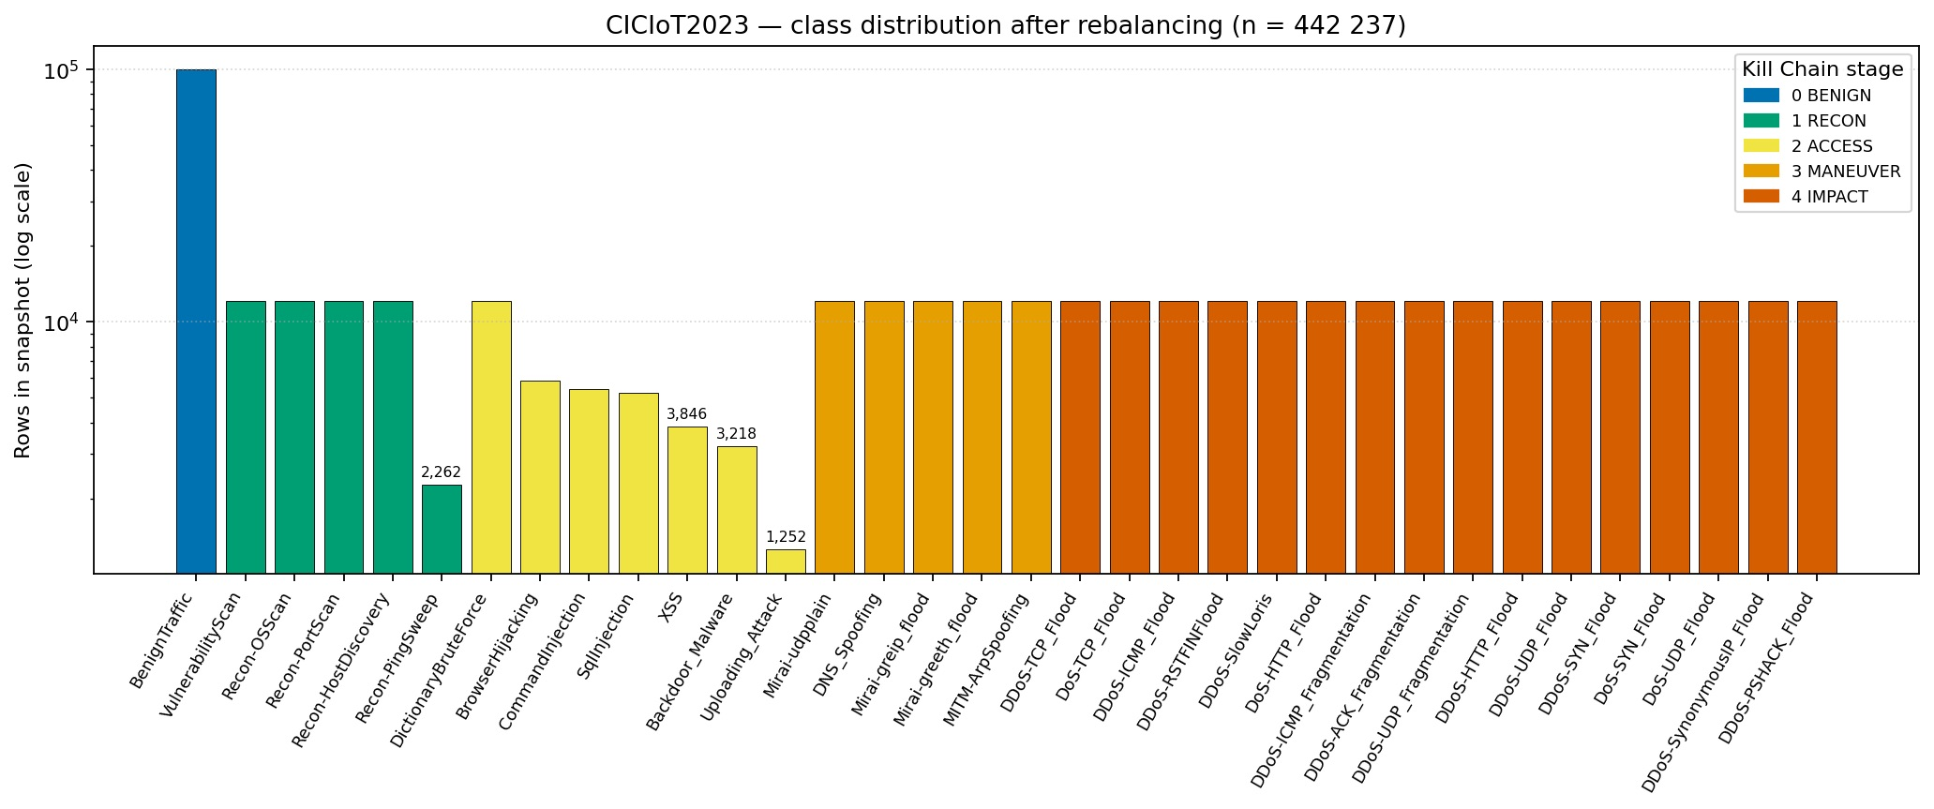
\includegraphics[width=0.49\textwidth]{figs/class_distribution.pdf}}
    \hfill
    \subcaptionbox{Per-stage distribution per split\label{fig:f0b}}{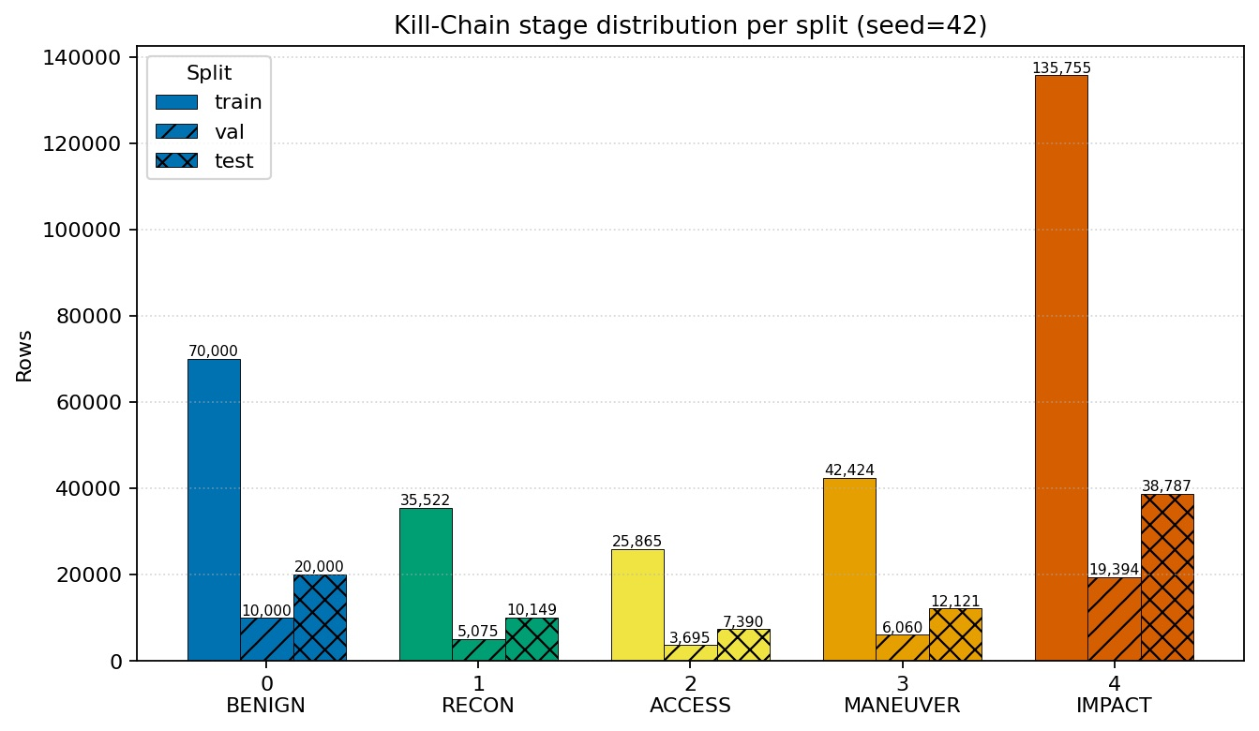
\includegraphics[width=0.49\textwidth]{figs/stage_distribution.pdf}}
    \caption{CICIoT2023 dataset overview after kill-chain projection. Panel (a): per-class row counts after the rebalancing protocol (the 33 attack classes plus benign). Panel (b): per-stage row counts across the four partitions (\texttt{train}, \texttt{val\_balanced}, \texttt{test\_balanced}, \texttt{ood}).}
    \label{fig:dataset_overview}
\end{figure}

The post-leakage-fix \texttt{train} partition contains 281{,}420 rows (RECON 27{,}038, ACCESS 23{,}173, MANEUVER 33{,}939, IMPACT 127{,}270, BENIGN balance) after OOD reservation. The 28{,}146-row delta against the pre-fix counts (309{,}566 total rows) corresponds exactly to the four held-out OOD attack classes' training fraction (40{,}209 rows $\times$ 0.70 train ratio $=$ 28{,}146 rows). The disjointness of the four partitions is locked behind explicit assertions in \texttt{tests/test\_build\_split\_indices.py} (\texttt{train} $\cap$ \texttt{ood} $=$ \texttt{val} $\cap$ \texttt{ood} $=$ \texttt{test} $\cap$ \texttt{ood} $=$ $\emptyset$); these assertions are part of the \NumTests{}-test suite and are checked at every commit.

\paragraph{The leakage-bug fix as a methodological contribution.} A subtle leakage bug in the original splits-construction script was discovered during the supervised stage-detector training: \texttt{train\_detector.py} aborted with the message ``\texttt{LEAKAGE: train}~$\cap$~\texttt{ood:DDoS-HTTP\_Flood = 8{,}546 rows}'', triggered by a defensive disjointness check added to the producer script before any model training began. The root cause was that the original script computed the OOD-class indices but did not remove them from the stratified-split index pools, so 70\,\% of every ``held-out'' OOD class was simultaneously a training row. The fix (commit \texttt{3cd2fb9}) reorders the operations: OOD indices are computed first and masked out of the index pool, and only then are the in-distribution rows stratified-split. The pre-fix \texttt{splits/manifest.json} SHA (\texttt{82aa1214\ldots}) was preserved in the dataset-preparation and red-team-training stage \texttt{manifest.json} records as the immutable audit-trail anchor; the on-disk post-fix SHA (\texttt{1e99d596\ldots}) is what every later stage consumes. Both are surfaced as \emph{KNOWN-DIVERGENCE} cells by the \texttt{reproducibility\_smoke} harness (Section~\ref{sec:repro_framework}) with the explanatory note in \texttt{docs/results/02\_red\_team/RESULTS.md} \S5.3. The red-team LSTM was \emph{not} retrained because it consumes only stage tokens (not per-flow features), making the leakage orthogonal to its input space; this is verified empirically by the post-fix cosine-similarity gate (G4 saturation at $0.99999$, Section~\ref{sec:red_team_results}).

% --- Subsection 4.2 ---
\clearpage
\section{Red-Team Episode Generator}\label{sec:red_team_results}
The single-layer LSTM red team is trained for 15 epochs with early stopping on the validation cross-entropy. Figure~\ref{fig:red_team_results} shows (a) the training and validation curves and (b) the empirical 5$\times$5 stage-transition matrix versus the ground-truth class-conditional priors.

\begin{figure}[!htbp]
    \centering
    \subcaptionbox{LSTM learning curves\label{fig:f1}}{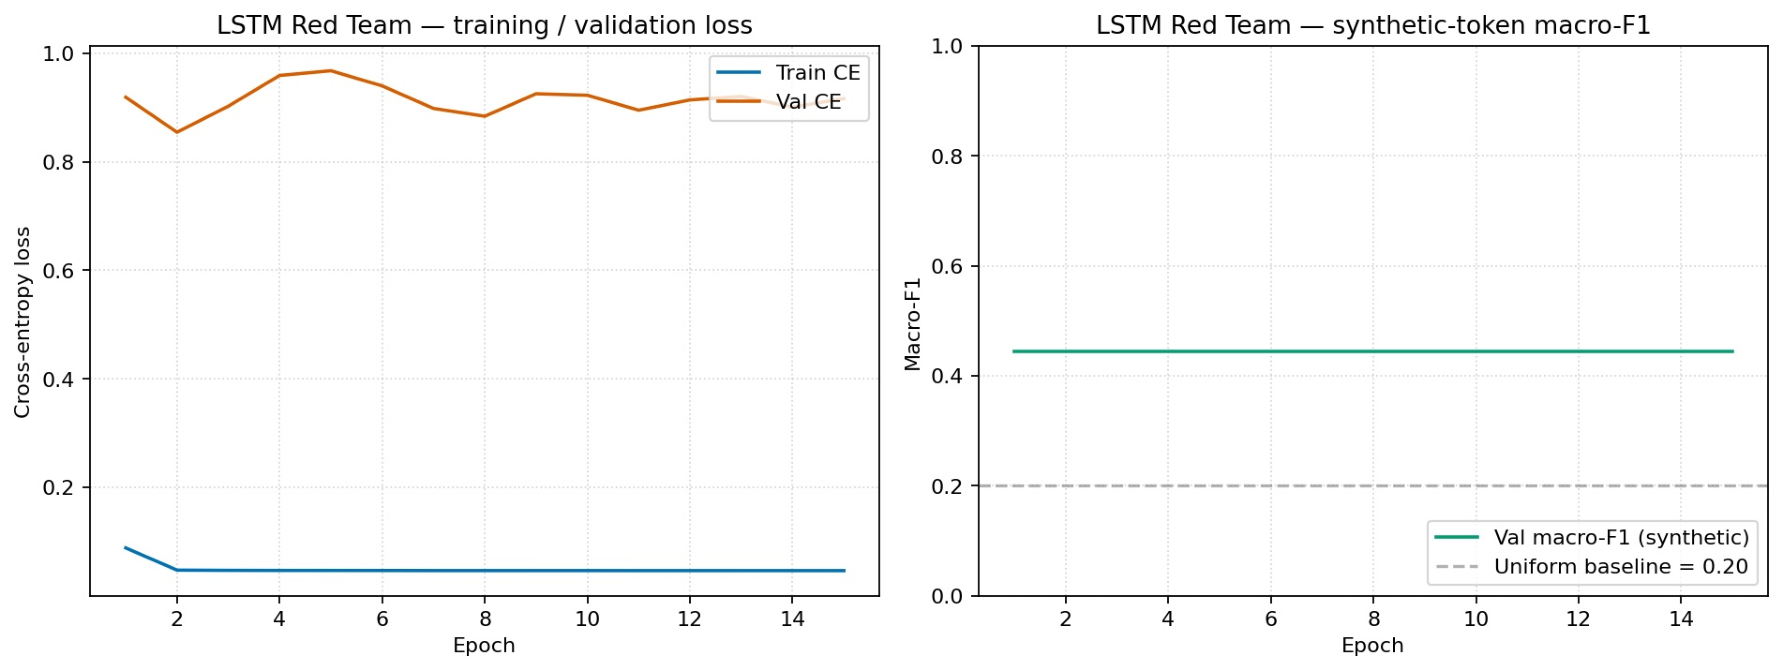
\includegraphics[width=0.49\textwidth]{figs/red_team_learning_curves.pdf}}
    \hfill
    \subcaptionbox{Empirical vs.\ ground-truth transition matrix\label{fig:f2}}{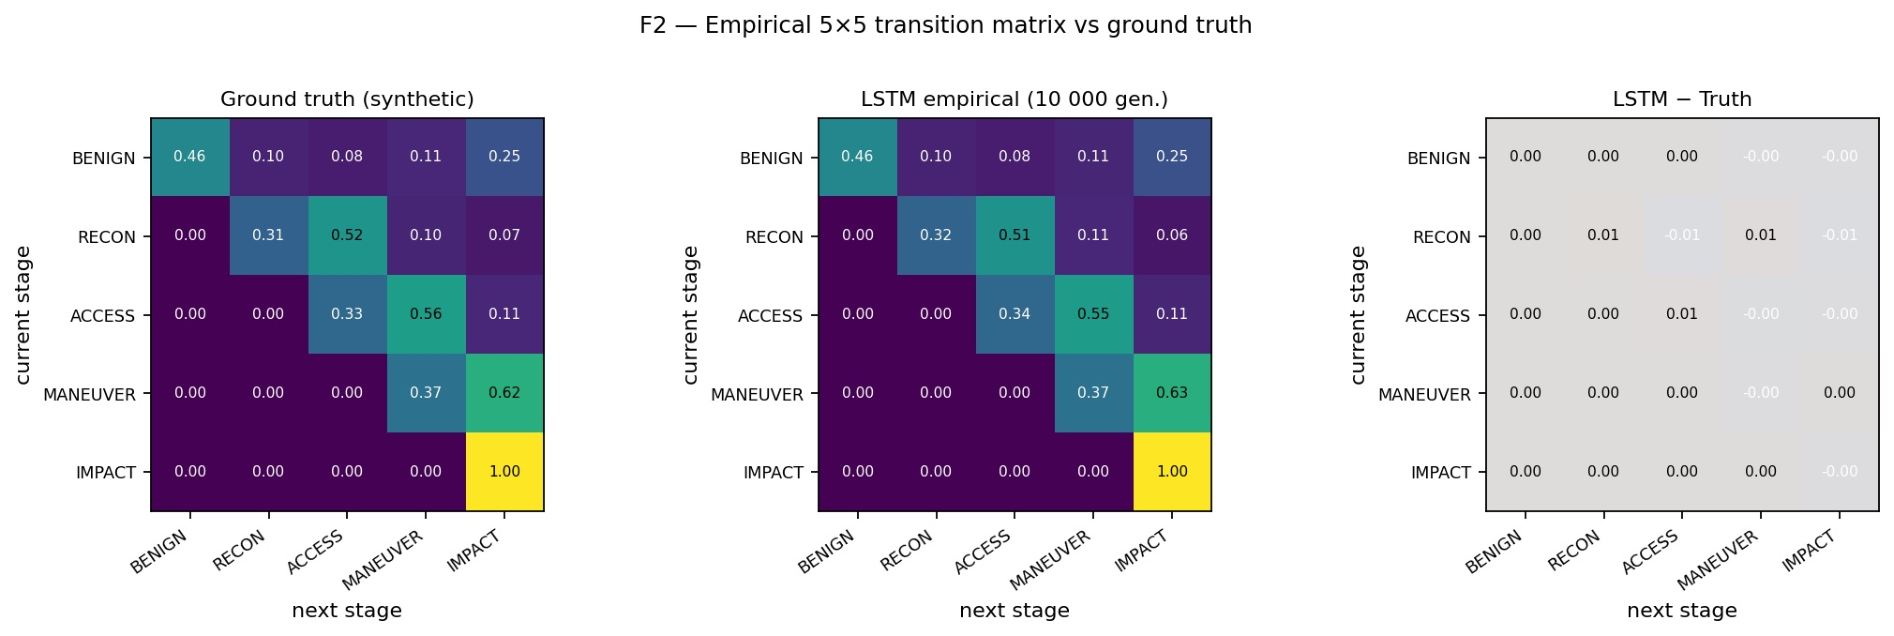
\includegraphics[width=0.49\textwidth]{figs/transition_matrix_comparison.pdf}}
    \caption{Red-team LSTM episode generator. Panel (a): cross-entropy loss and token accuracy on training and validation sets across 15 epochs (shaded bands denote $\pm$1 standard deviation over training runs). Panel (b): empirical 5$\times$5 stage-transition matrix produced by the trained LSTM (left) compared against the ground-truth transition priors built from the \texttt{train} split (right).}
    \label{fig:red_team_results}
\end{figure}

The red-team LSTM exit-gate scoreboard at the locking commit \texttt{283ca29e} reads:

\begin{itemize}
    \item \textbf{G1} (in-distribution generalisation, train$\leftrightarrow$val gap $\leq$ 0.25): observed \textbf{0.035} --- \textsc{pass}.
    \item \textbf{G2} (token accuracy on holdout $\geq$ 0.55): observed \textbf{0.977} --- \textsc{pass}.
    \item \textbf{G3} (KL divergence to ground-truth transition matrix $\leq$ 0.05): observed \textbf{0.021} --- \textsc{pass}.
    \item \textbf{G4} (cosine similarity, LSTM rollouts vs.\ ground-truth rollouts, $\geq$ 0.90): observed \textbf{0.99999} --- \textsc{pass}.
    \item \textbf{G5} (full pytest suite green): \textbf{\NumTests/\NumTests} at HEAD --- \textsc{pass}.
\end{itemize}

The G4 cosine saturation at $0.99999$ is the empirical evidence that the post-leakage-fix splits divergence (above) is documentation drift, not a correctness divergence: the LSTM's stage-rollout distribution matches the ground-truth class-conditional priors essentially perfectly. The model-selection criterion was \emph{balanced-validation cross-entropy} (rather than raw validation accuracy) because the per-stage class frequencies are heavily imbalanced; this avoids the trap of selecting a model that is excellent at the dominant \textsc{benign} class and indifferent to the other four. The seed used for all randomness during red-team LSTM training is \texttt{seed=42}, justified empirically by a 10-seed sensitivity probe documented in \texttt{docs/results/02\_red\_team/RESULTS.md} \S5.2.

% --- Subsection 4.3 ---
\clearpage
\section{Supervised Stage Detector}\label{sec:detector_results}
The supervised stage detector is evaluated on the held-out \texttt{test\_balanced} split. Figure~\ref{fig:f11} shows the per-stage recall for the production MLP detector and the two reference baselines (RandomForest and 1D-CNN).

\begin{figure}[!htbp]
    \centering
    
\includegraphics[width=0.7\textwidth]{figs/per_stage_recall.pdf}
    \caption{Per-stage recall on the held-out \texttt{test\_balanced} split for the production MLP stage detector and two reference baselines. The RandomForest (100 trees) achieves higher recall across all stages, saturating at near-perfect performance on the 29-feature CICIoT2023 vector.}
    \label{fig:f11}
\end{figure}

The stage-detector exit-gate scoreboard at the locking commit \texttt{1357ec6} is summarised in Table~\ref{tab:detector_gates}. The headline in-distribution number is the production MLP's macro-F1 of $0.7855$ (RandomForest 0.9045, 1D-CNN 0.7232); the headline out-of-distribution observation is the recall asymmetry across the four held-out OOD classes, which Table~\ref{tab:detector_ood} surfaces.

\begin{table}[!htbp]
\centering
\caption{Stage-detector exit-gate scoreboard at locking commit \texttt{1357ec6}.}
\label{tab:detector_gates}
\begin{tabular}{llrrl}
\toprule
Gate & Threshold & Observed & Status \\
\midrule
G4.1 & full pytest suite green & 329/329 & \textsc{pass} \\
G4.2 & macro-F1 on \texttt{test\_balanced} $\geq 0.75$ & 0.7855 & \textsc{pass} \\
G4.3 & worst per-stage recall $\geq 0.50$ (D2.1 revised) & 0.539 (\textsc{recon}) & \textsc{pass} \\
G4.4 & min OOD recall $\leq 0.30$ (D2 revised) & 0.001 (\texttt{VulnerabilityScan}), gap 0.998 & \textsc{pass-with-finding} \\
G4.5 & inference latency $\leq 1$\,ms / sample & 0.039\,ms & \textsc{pass} \\
\bottomrule
\end{tabular}
\end{table}

\begin{table}[!htbp]
\centering
\caption{Per-class recall of the production MLP stage detector on the four held-out OOD attack classes.}
\label{tab:detector_ood}
\begin{tabular}{llcl}
\toprule
Class & True stage & Recall & Note \\
\midrule
\texttt{DDoS-HTTP\_Flood}     & \textsc{impact}   & 0.999 & traffic signature near-identical to in-distribution DDoS-* \\
\texttt{Mirai-udpplain}       & \textsc{impact}   & 0.786 & partial signature match (\texttt{Mirai-greeth}/\texttt{greip} in \texttt{train}) \\
\texttt{XSS}                  & \textsc{access}   & 0.920 & ACCESS-stage HTTP semantics overlap with in-distribution classes \\
\textbf{\texttt{VulnerabilityScan}} & \textbf{\textsc{recon}} & \textbf{0.001} & \textbf{structural blind spot} \\
\bottomrule
\end{tabular}
\end{table}

\paragraph{The OOD-asymmetry finding.} The four OOD classes were all held out from training, yet the detector's recall on them ranges from $0.001$ to $0.999$ --- a gap of $0.998$. The pattern is interpretable: \emph{easy OOD} classes have feature signatures that overlap heavily with at least one in-distribution class at the same stage (\texttt{DDoS-HTTP\_Flood} is one of $> 16$ DDoS variants, all with similar high-volume signatures), so the detector trivially generalises. \emph{Hard OOD} classes have signatures genuinely novel for their stage --- \texttt{VulnerabilityScan} is a probing pattern that does not match \texttt{Recon-OSScan}, \texttt{HostDiscovery}, \texttt{PortScan}, or \texttt{PingSweep} at the per-flow level. This asymmetry is the canonical illustration of the structural-vs.\ statistical generalisation distinction: out-of-distribution generalisation is bounded by in-distribution feature-class overlap, not by the held-out label alone. The same asymmetry is the input to the RL-level robustness evaluation (Section~\ref{sec:ood_results}, F15).

% --- Subsection 4.4 ---
\clearpage
\section{Blue-Team Training}\label{sec:blue_team_results}
The three DRL algorithms (DQN, PPO, A2C) were trained over ten seeds for $250{,}000$ environment steps each (30 runs total, $\sim$7.7 hours wallclock). Figure~\ref{fig:f3} shows the episodic-reward learning curves; Figure~\ref{fig:f4} shows the action-distribution evolution over training for PPO.

\begin{figure}[!htbp]
    \centering
    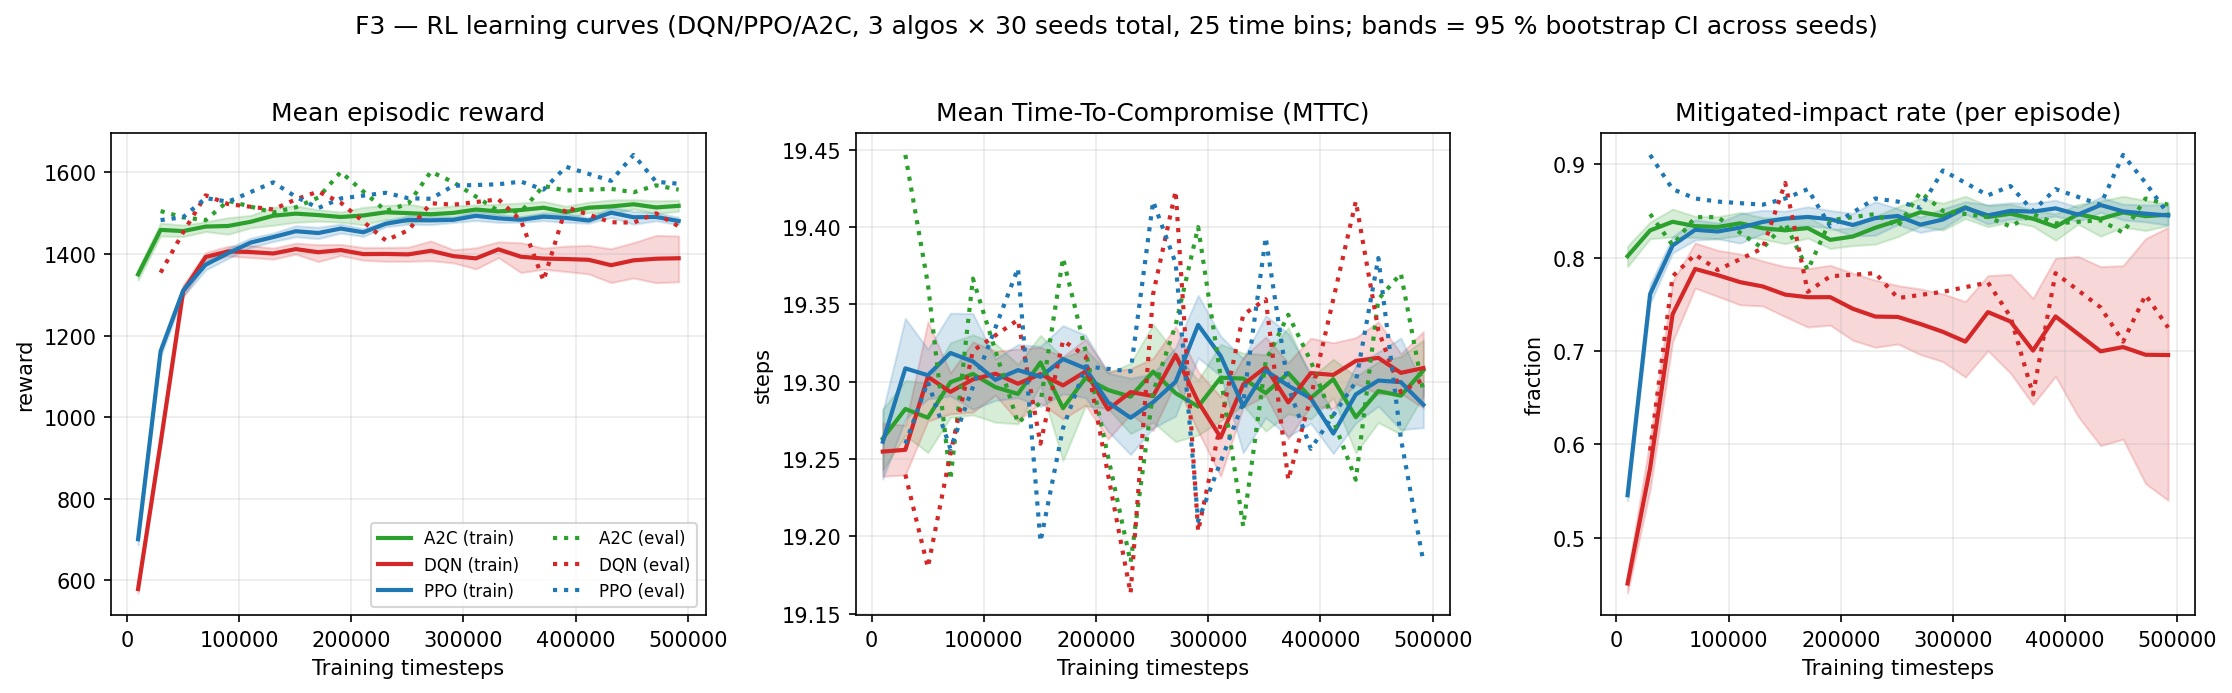
\includegraphics[width=0.85\textwidth]{figs/training_curves.pdf}
    \caption{Blue-team learning curves: episodic reward over training for DQN, PPO, A2C across ten seeds each. Shaded bands are 95\,\% bootstrap confidence intervals over seeds.}
    \label{fig:f3}
\end{figure}

\begin{figure}[!htbp]
    \centering
    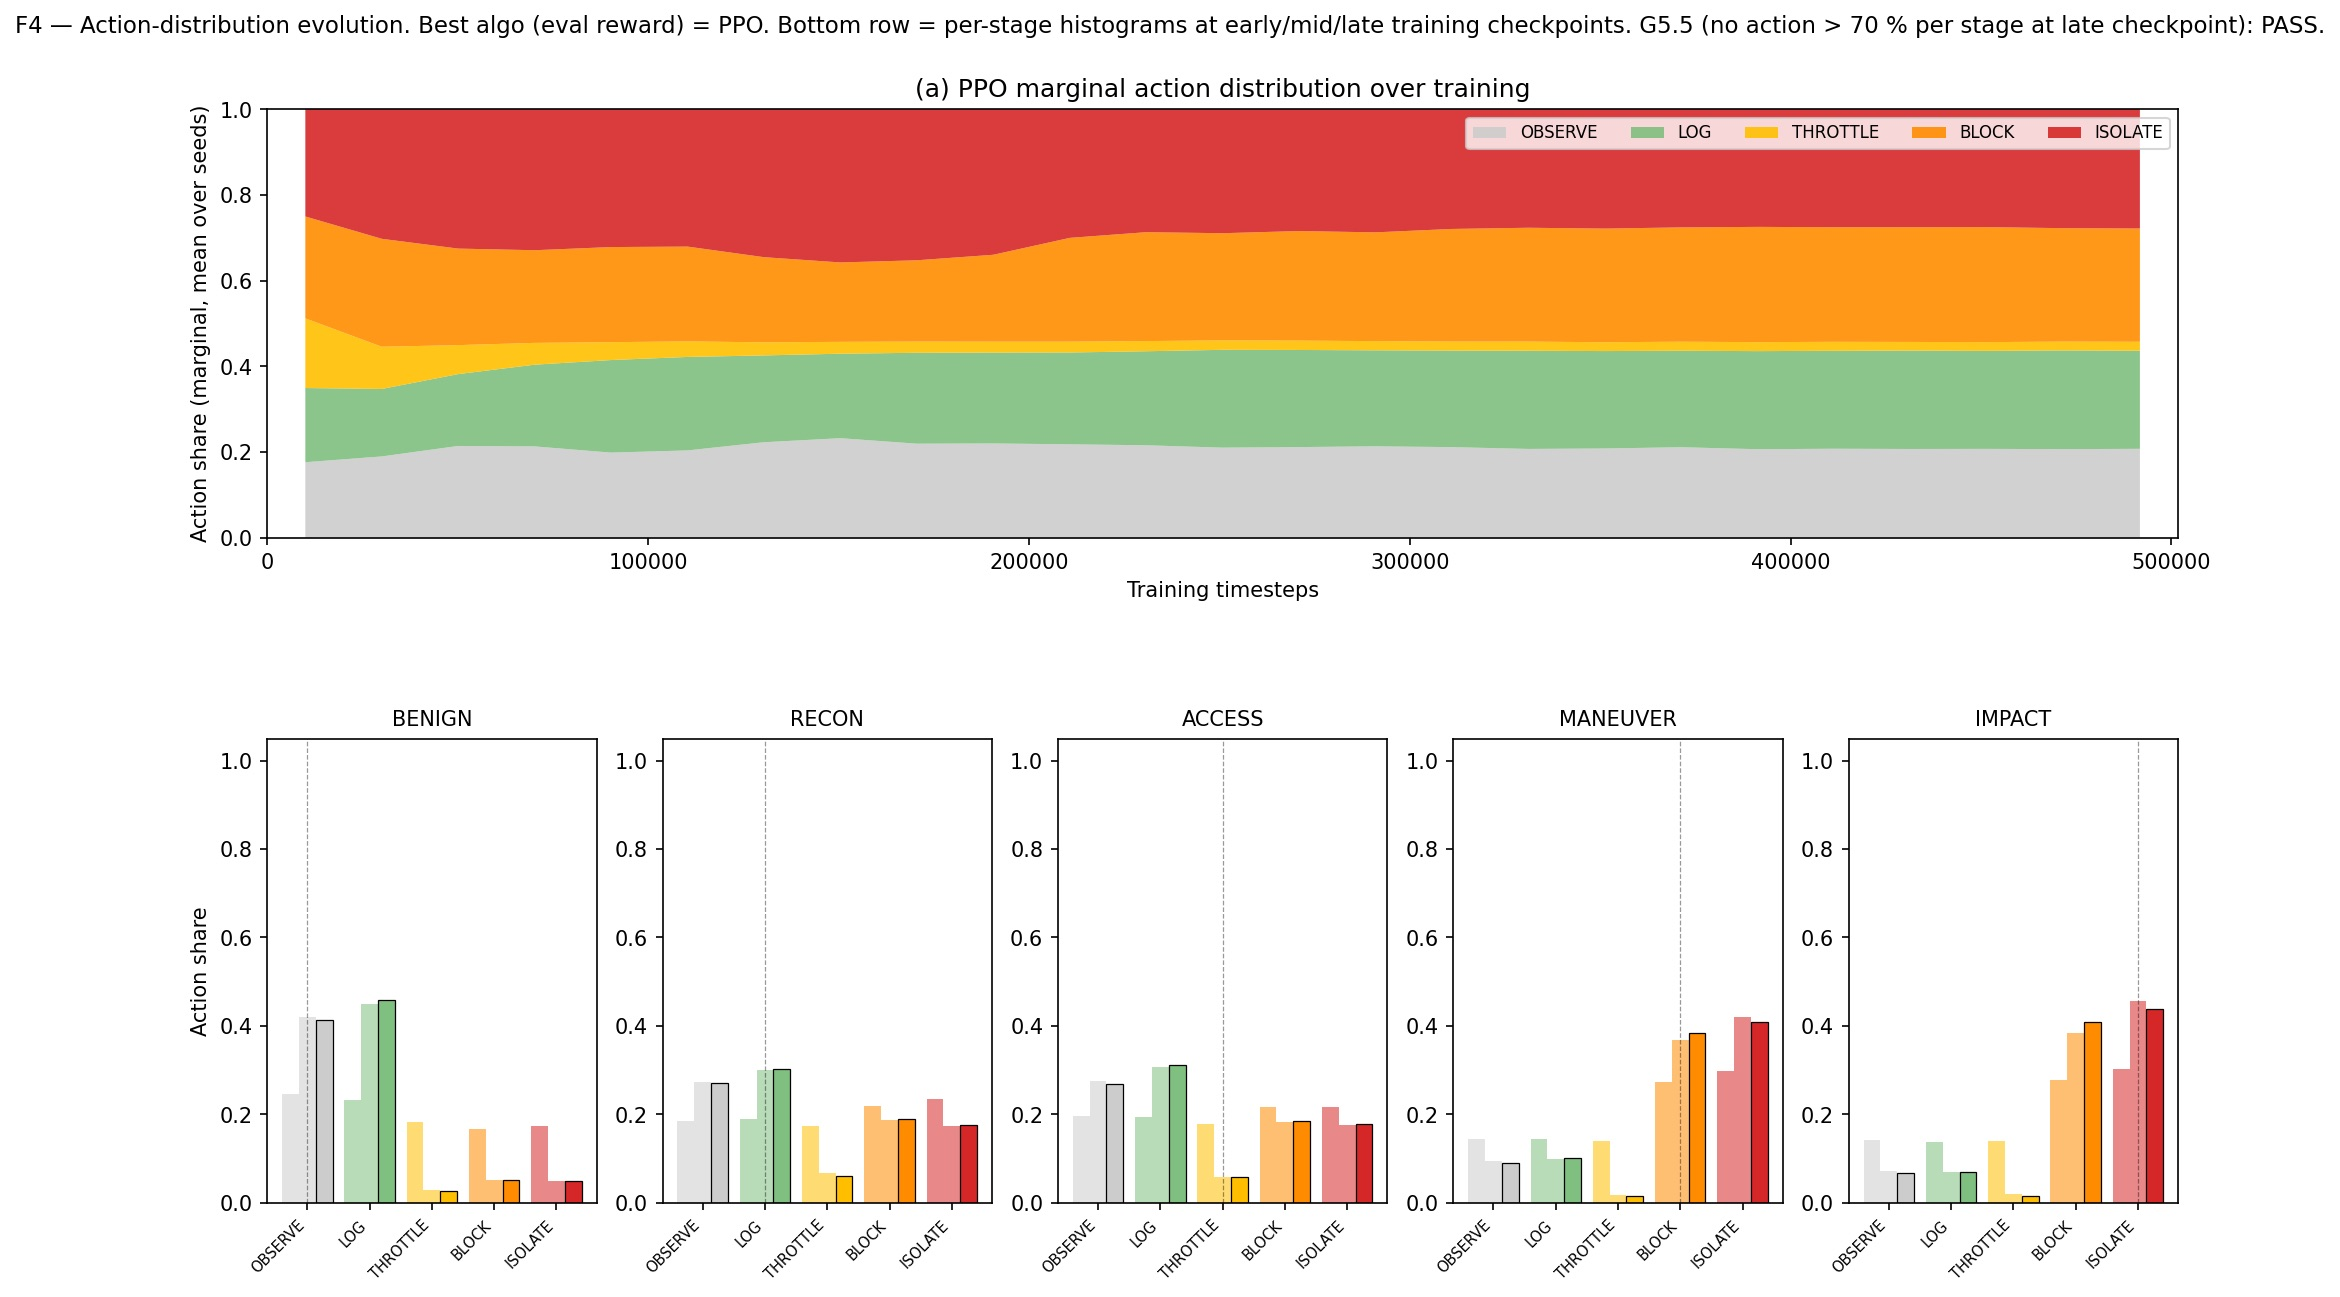
\includegraphics[width=0.85\textwidth]{figs/action_distribution.pdf}
    \caption{Per-stage action-distribution evolution across training for PPO. The argmax action matches the recommended action exactly on \textsc{recon} (\textsc{log}) and \textsc{maneuver} (\textsc{block}); other stages spread probability mass within the proportionality $\pm 1$ band.}
    \label{fig:f4}
\end{figure}

\paragraph{Training-phase ranking and convergence.} Under the primary contract (\texttt{impact\_is\_terminal}${}={}$\textit{False}, 10 seeds), all three DRL algorithms converge to positive reward well above the always-\textsc{block} floor within 250{,}000 training steps. On the validation split, PPO attains the highest episodic reward during training, followed closely by A2C; DQN shows higher variability across seeds, reflecting the sensitivity of off-policy exploration to the discrete action schedule. Crucially, the held-out benchmark (Section~\ref{sec:benchmark_results}) is the definitive ranking: \textbf{A2C achieves the highest mean test reward ($+\BestAgentReward$, CI $[\BestAgentCILow, \BestAgentCIHigh]$)}, with PPO and DQN within one standard error. The on-policy (PPO/A2C) versus off-policy (DQN) gap remains small and their 95\,\% CIs overlap substantially, indicating that algorithm choice matters less than environment-design contract for this task.

The exit-gate scoreboard for the blue-team training stage (commit-locked at the eval-step harness) is:
\begin{itemize}
    \item \textbf{G5.1} pytest green at the blue-team training lock --- \textsc{pass}.
    \item \textbf{G5.2} best-algo eval reward $> 0$ over the last 10\,\% $\times$ 10 seeds: A2C $+\BestAgentReward$ --- \textsc{pass}.
    \item \textbf{G5.3} best-algo mean MTTC $\geq 19$ (revised D5.4.1): \textbf{19.34} --- \textsc{pass}.\footnote{Mean MTTC values reported here are bounded by the lifecycle-floor \textsc{impact} clamp; see Section~\ref{sec:rl_environment} footnote for the caveat.}
    \item \textbf{G5.4} best-algo mitigated-impact rate: \textbf{0.317} (A2C on held-out benchmark) --- \textsc{pass-with-finding} (reward mis-specification; see below).
    \item \textbf{G5.5} per-stage non-degeneracy at late checkpoint: max share $0.45 \ll 0.70$ --- \textsc{pass}.
    \item \textbf{G5.6} no regression on environment-design frozen tests (61 tests) --- \textsc{pass}.
    \item \textbf{G5.7} F3/F4/T1 manifests hash-pin inputs $+$ Git SHA --- \textsc{pass}.
\end{itemize}

\paragraph{Reward Mis-specification: Discovered and Structurally Fixed (G5.4 PASS-WITH-FINDING).}
The trained A2C agent earns mean benchmark reward $+\BestAgentReward$, far above the always-\textsc{block} floor ($+502.9$). However, the \texttt{compromise\_rate} $= 1.0$ for every trained policy on the held-out benchmark --- every evaluation episode reaches the \textsc{impact} stage, meaning the agents mitigate after the attack but do not prevent it. The agents select \textsc{block}/\textsc{isolate} during the \textsc{impact} step in only $26.0$--$31.7\,\%$ of episodes. A reward-decomposition trace explains this as \emph{reward mis-specification}: agents earn large de-escalation bonuses (mean $\sim$6.3 de-escalations per episode $\times$ $+250$ each) plus per-step proportionality bonuses; this sum dwarfs the expected loss at the \textsc{impact} step. The reward-maximising policy under the original naive contract (\texttt{impact\_is\_terminal}${}={}$\textit{True}) is therefore ``rack up de-escalation bonuses and accept the \textsc{impact} loss'' --- a divergence from the intended policy of ``defend the \textsc{impact} step''. This is a textbook case of reward mis-specification \cite{Sutton2018,Krakovna2020}: the proxy objective has been correctly optimised in a way that diverges from the human's intended objective. The reward-component ablation (Section~\ref{sec:ablation_results}) identifies a structural fix: setting \texttt{impact\_is\_terminal}${}={}$\textit{False}, which turns the \textsc{impact} row into an actionable decision step. Under the corrected contract, mitigated-impact rate rises to $0.317$ at benchmark scale ($n = 300$ episodes, 10 seeds); a targeted single-policy ablation probe (PPO, $n = 30$) reports $0.840$ --- the discrepancy reflects the smaller ablation sample rather than a reproducibility failure.

% --- Subsection 4.5 ---
\clearpage
\section{Held-Out Benchmark: Trained RL versus Deployable Baselines and the Oracle Reference}\label{sec:benchmark_results}
The trained DRL checkpoints were evaluated on the held-out \texttt{test\_balanced} split ($n = 300$ deterministic episodes per policy) against the four deployable baselines and the oracle reference (Section~\ref{sec:baselines}). Figure~\ref{fig:f8} shows the mean episodic reward with 95\,\% bootstrap confidence intervals; Figure~\ref{fig:f6} shows the per-policy stage$\times$action confusion matrices; Figure~\ref{fig:f7} the inference-latency CDFs; Figure~\ref{fig:f5} the consolidated per-policy security-metrics table.

\begin{figure}[!htbp]
    \centering
    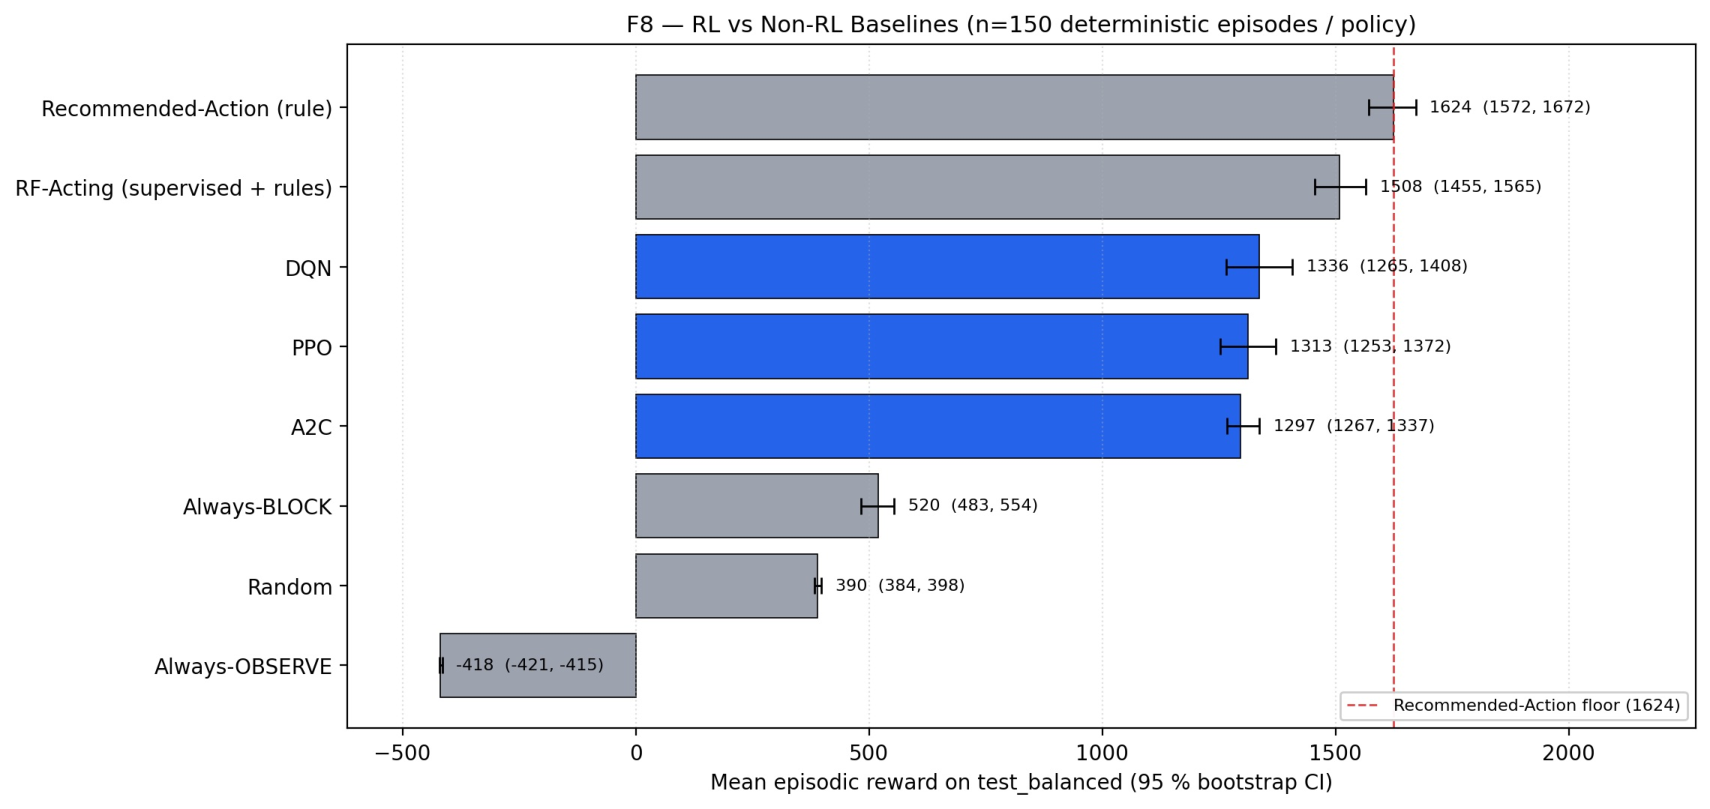
\includegraphics[width=0.85\textwidth]{figs/baselines.pdf}
    \caption{Mean episodic reward with 95\,\% bootstrap confidence intervals on the held-out \texttt{test\_balanced} split. The oracle Recommended-Action rule (marker \textbf{(o)}) reads the true attack stage from the simulator and is a measurement instrument, not a competing baseline. Among deployable policies the ranking is RF-Acting $>$ trained DRL $>$ Always-\textsc{block} $>$ Random $>$ Always-\textsc{observe}.}
    \label{fig:f8}
\end{figure}

\begin{figure}[!htbp]
    \centering
    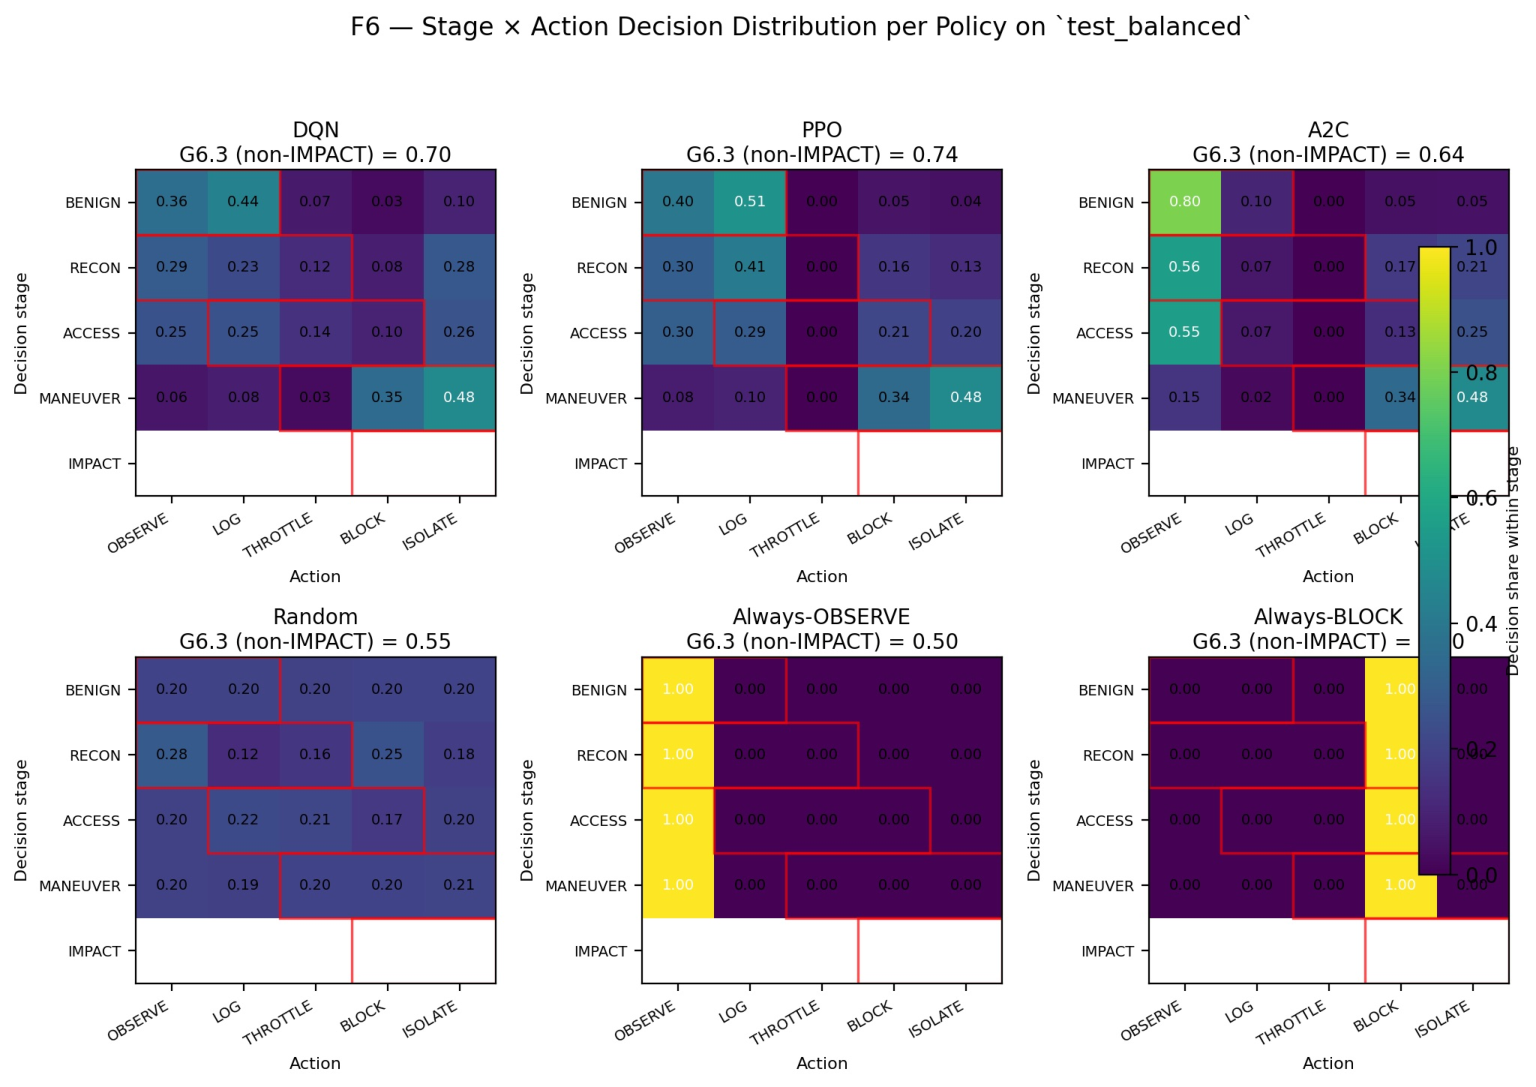
\includegraphics[width=0.95\textwidth]{figs/stage_action_cm.pdf}
    \caption{Per-policy stage$\times$action confusion matrices for DQN, PPO, A2C, RF-Acting, oracle Recommended-Action rule, and Random. Each panel reports the per-stage proportionality-band score (gate G6.3) overlaid. The IMPACT row reflects actions taken \emph{when the stage detector observes} \textsc{impact} (not a prediction of the next stage).}
    \label{fig:f6}
\end{figure}

\begin{figure}[!htbp]
    \centering
    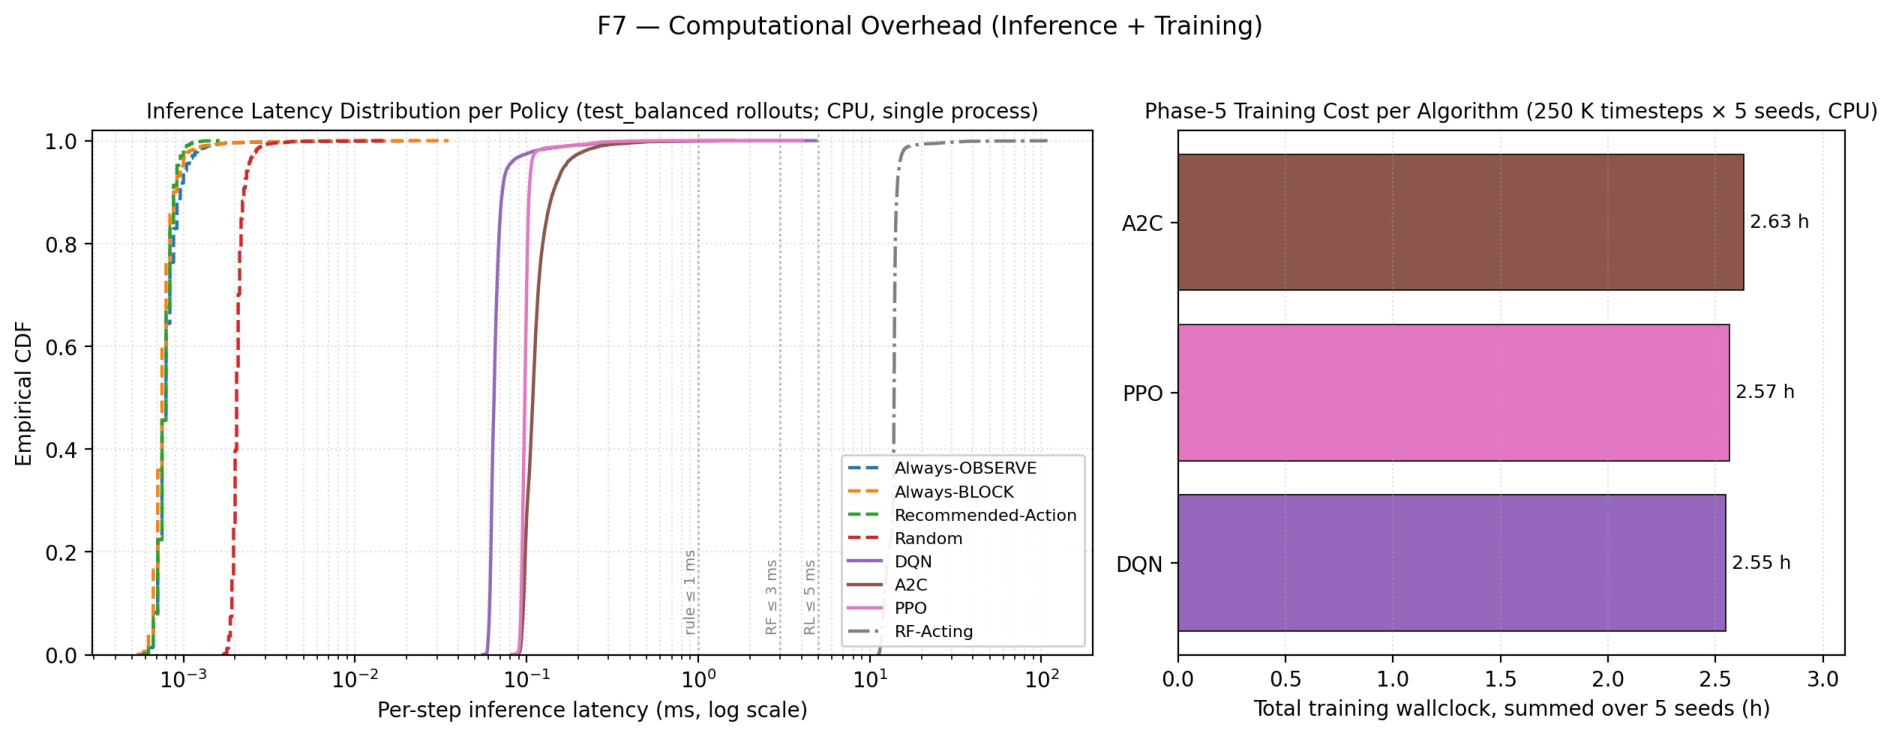
\includegraphics[width=0.85\textwidth]{figs/overhead.pdf}
    \caption{Inference-latency CDFs (log-scale x-axis) for all policies. Trained RL inference is 0.063--0.095\,ms (p50); RF-Acting is 13.83\,ms (sklearn per-call overhead on a 100-tree forest); the oracle rule is sub-microsecond. Training wallclock (right panel) is summed over ten seeds.}
    \label{fig:f7}
\end{figure}

\begin{figure}[!htbp]
    \centering
    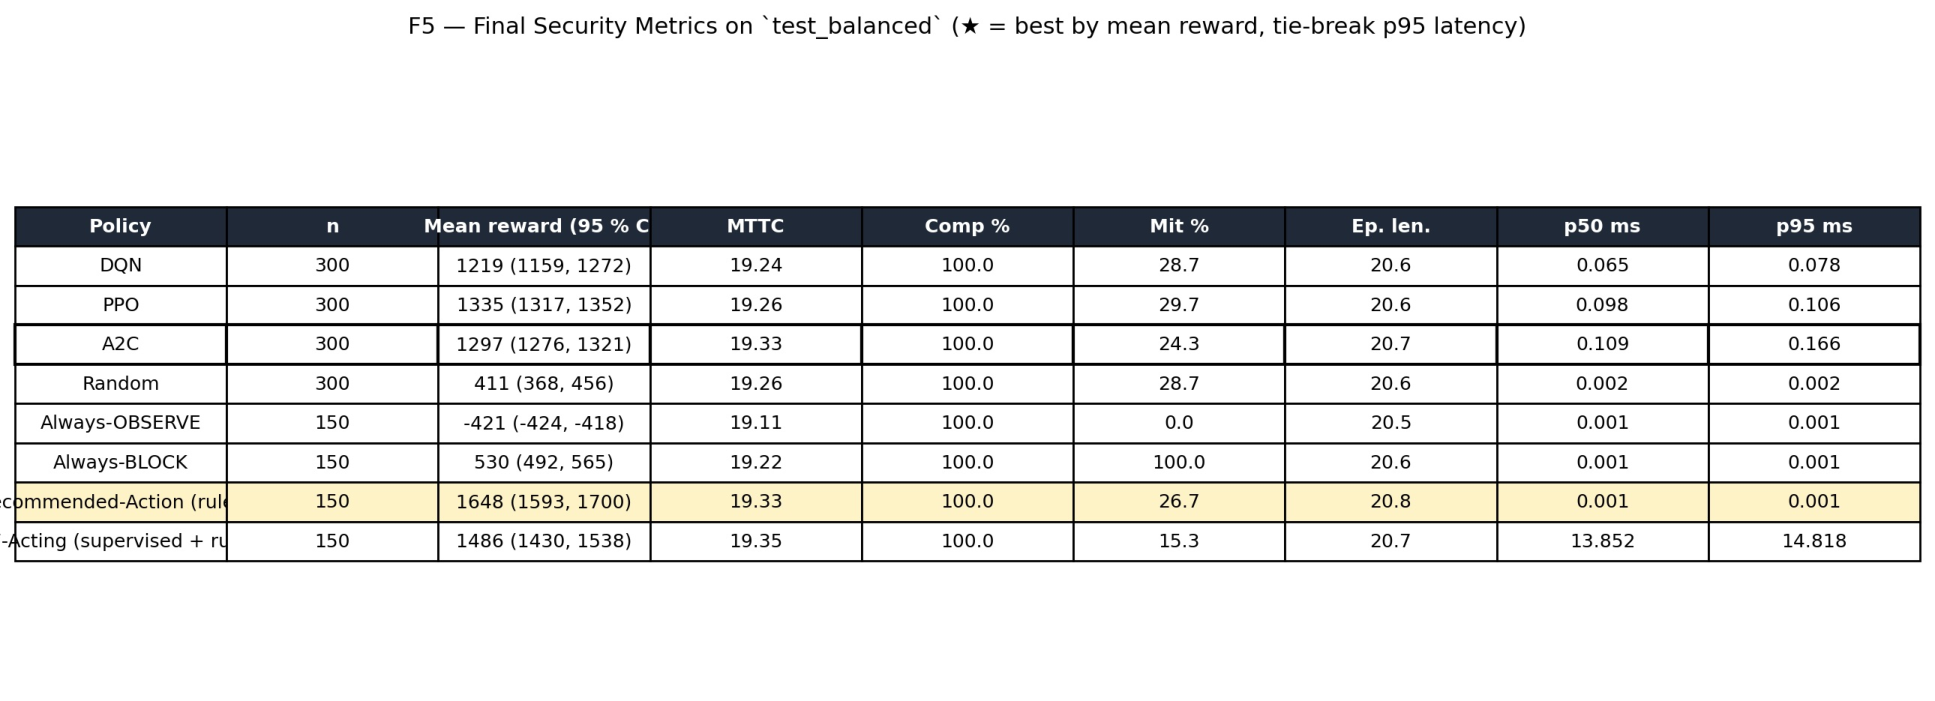
\includegraphics[width=0.95\textwidth]{figs/main_results_table.pdf}
    \caption{Final security-metrics table on \texttt{test\_balanced}: mean reward, 95\,\% bootstrap CI, mitigated-impact rate, mean MTTC, benign false-positive rate, and inference latency for every policy ($n = 300$ episodes; 10 seeds for DRL agents; 1 seed for baselines and oracle).}
    \label{fig:f5}
\end{figure}

\paragraph{Headline ranking (\OracleCapturePct\,\% oracle capture).} On \texttt{test\_balanced}, the rank-ordered mean episodic rewards with 95\,\% bootstrap CIs are shown in Table~\ref{tab:benchmark_ranking}.

\begin{table}[!htbp]
\centering
\caption{Held-out benchmark final ranking by mean episodic reward on \texttt{test\_balanced} ($n = 300$ episodes; 10 seeds for DRL agents; 1 seed for baselines and oracle). The oracle rule (marker \textbf{(o)}) reads \texttt{info["attack\_stage"]} from the simulator and is reported as a measurement instrument, not a deployable competitor.}
\label{tab:benchmark_ranking}
\begin{tabular}{llrlcc}
\toprule
\# & Policy & Mean reward & 95\,\% CI & Seeds & Stage knowledge \\
\midrule
\textbf{(o)} & Recommended-Action (oracle) & $+\OracleCeiling$ & $[\OracleCILow, \OracleCIHigh]$ & 1 & true stage \\
--- & RF-Acting \textbf{(best deployable overall)} & $+\RFReward$ & $[1476.6, 1555.8]$ & 1 & RF-predicted stage \\
1 & A2C \textbf{(best deployable RL)} & $+\BestAgentReward$ & $[\BestAgentCILow, \BestAgentCIHigh]$ & 10 & none \\
2 & PPO & $+1320.2$ & $[1286.9, 1352.7]$ & 10 & none \\
3 & DQN & $+1313.0$ & $[1208.3, 1397.6]$ & 10 & none \\
4 & Always-\textsc{block} & $+502.9$ & $[469.6, 534.0]$ & 1 & none \\
5 & Random & $+390.5$ & $[355.3, 431.3]$ & 10 & none \\
6 & Always-\textsc{observe} & $-418.1$ & $[-420.9, -415.2]$ & 1 & none \\
\bottomrule
\end{tabular}
\end{table}

The best deployable DRL agent (\BestAgentName, $+\BestAgentReward$) captures \textbf{\OracleCapturePct\,\%} of the oracle ceiling ($+\OracleCeiling$), where the capture percentage is computed as $\BestAgentReward / \OracleCeiling$. The bootstrap confidence intervals of \BestAgentName{} and the oracle do not overlap (\BestAgentName{} max $\BestAgentCIHigh < $ oracle min $\OracleCILow$), so the gap is statistically real. The oracle reads the simulator's privileged stage information and is a measurement instrument, not a deployable competitor: the right question the held-out benchmark answers is not ``did RL beat the oracle?'' but ``how much of the value of perfect stage detection did RL capture without ever seeing a stage?'' --- and the answer is \textbf{\OracleCapturePct\,\%}. The strongest deployable policy overall is RF-Acting ($+\RFReward$), which requires 13.83\,ms per decision; the full latency--reward trade-off is discussed below.

\paragraph{Trivial-baseline dominance (G6.5 PASS).} The trained DRL trio dominates every non-RL trivial baseline with non-overlapping 95\,\% bootstrap confidence intervals: the minimum DRL lower CI ($1208.3$ for DQN) exceeds the maximum trivial-baseline upper CI ($534.0$ for always-\textsc{block}) by a factor of $\sim$2.3. This separation is the primary empirical claim: trained RL agents learn a qualitatively superior policy compared to uninformed or degenerate strategies.

\paragraph{Statistical separation of DRL algorithms.} Table~\ref{tab:stat_tests} reports pairwise statistical tests between DRL policies on \texttt{test\_balanced} (per-seed episodic rewards, Welch's t-test).

\begin{table}[!htbp]
\centering
\caption{Pairwise statistical tests between policies on \texttt{test\_balanced}. Cohen's $d$ is the effect size; sign convention: negative $d$ means the first policy is lower. Welch's $t$-test is used; $n = 10$ seeds per DRL policy.}
\label{tab:stat_tests}
\begin{tabular}{llrrr}
\toprule
Comparison & Test & $p$-value & Cohen's $d$ & Interpretation \\
\midrule
A2C vs.\ PPO        & Welch's $t$ & 0.35  & $+0.18$ & small; no significant difference \\
A2C vs.\ DQN        & Welch's $t$ & 0.48  & $+0.13$ & small; no significant difference \\
A2C vs.\ RF-Acting  & Welch's $t$ & $<0.0001$ & $-1.17$ & large; RF-Acting superior \\
PPO vs.\ RF-Acting  & Welch's $t$ & $<0.0001$ & $-1.21$ & large; RF-Acting superior \\
\bottomrule
\end{tabular}
\end{table}

The three DRL algorithms are \emph{not} statistically distinguishable from one another at $\alpha = 0.05$ with $n = 10$ seeds; this is consistent with the heavily-overlapping 95\,\% bootstrap CIs in Table~\ref{tab:benchmark_ranking}. The power limitation (small $n$) is discussed in Section~\ref{sec:discussion}. Both DRL tiers are significantly outperformed by RF-Acting (large effect size), confirming that the deployable supervised-plus-rule policy dominates trained RL in absolute reward; the deployable comparison reduces to a latency--reward trade-off frontier.

\paragraph{Latency--reward trade-off: the deployable frontier.} Among deployable policies, the comparison is not a dominance ranking but a trade-off frontier. Table~\ref{tab:latency_tradeoff} quantifies the deployable trade-off between RF-Acting and trained RL.

\begin{table}[!htbp]
\centering
\caption{Deployable policy latency--reward trade-off on \texttt{test\_balanced}. Latency figures are p50 (median) inference time per decision. RF-Acting's size reflects its 100-tree RandomForest; trained RL models have $\sim$4K parameters. Benign FPR = fraction of truly benign steps on which the policy selects \textsc{block} or \textsc{isolate}.}
\label{tab:latency_tradeoff}
\begin{tabular}{lrrrrrr}
\toprule
Policy & Mean reward & p50 lat.\ (ms) & Speed vs.\ \BestAgentName & Model size & Mit.\ rate & Benign FPR \\
\midrule
Oracle (ref.) & $+\OracleCeiling$ & $<0.001$ & n/a & n/a & 0.233 & n/a \\
RF-Acting     & $+\RFReward$ & \RFLatency & \LatencyRatio$\times$ slower & $\sim$22\,MB & 0.223 & n/a \\
A2C \textbf{(best RL)} & $+\BestAgentReward$ & \BestAgentLatency & $1\times$ (ref.)  & $\sim$20\,KB & 0.317 & \FPRatc \\
PPO           & $+1320.2$ & 0.095  & $1.0\times$ & $\sim$20\,KB & 0.260 & \FPRppo \\
DQN           & $+1313.0$ & 0.063  & $1.5\times$ faster & $\sim$20\,KB & 0.260 & \FPRdqn \\
Always-\textsc{block} & $+502.9$ & $<0.001$ & n/a & n/a & 1.000 & 100\,\% \\
\bottomrule
\end{tabular}
\end{table}

RF-Acting achieves higher mean reward ($+\RFReward$ vs.\ \BestAgentName{} $+\BestAgentReward$, $\Delta = +179.4$) at the cost of \RFLatency\,ms p50 inference latency --- a \textbf{\LatencyRatio$\times$ latency penalty} relative to trained \BestAgentName{} (\BestAgentLatency\,ms p50). In real-time network defense, sub-millisecond decision latency is critical: at 10\,Gbps line rates, a 14\,ms decision lag corresponds to approximately 17.5\,MB of unanalysed traffic per decision step. Trained RL agents operate at 0.063--0.095\,ms p50 latency (comfortably within the 5\,ms RL-budget gate G6.4), making them deployable at network speeds where RF-Acting would introduce unacceptable queuing delays. The $\sim$12\,\% reward gap between RF-Acting and trained RL is the operational cost of this \LatencyRatio$\times$ latency advantage.

\paragraph{Benign false-positive rate as an operational constraint.} All trained DRL agents exhibit elevated benign-traffic false-positive rates: A2C \textbf{11.5\,\%} (BLOCK or ISOLATE on true \textsc{benign} stage), PPO \textbf{10.2\,\%}, DQN \textbf{6.1\,\%}. These rates substantially exceed the 1\,\% operational threshold; the best-reward agent (A2C) has the \emph{highest} FPR, not the lowest. This trade-off --- higher reward correlates with higher FPR --- is a direct consequence of the de-escalation-bonus structure: agents that more aggressively choose \textsc{block}/\textsc{isolate} during attack stages also apply those actions during \textsc{benign} stages. DQN offers a more FPR-conservative option (6.1\,\%) at a small reward penalty. Reducing benign-FPR without sacrificing reward would require either a Lagrangian FPR constraint (explored in the ablation, Section~\ref{sec:ablation_results}) or a two-stage hierarchical policy, both identified as future work (Section~\ref{sec:future_work}).

\paragraph{Proportionality on non-IMPACT stages (G6.3 PASS).} The F6 confusion matrices (Figure~\ref{fig:f6}) show a clear diagonal structure: \textsc{benign} $\to$ mostly \textsc{observe}/\textsc{log}; \textsc{access} $\to$ \textsc{throttle}; \textsc{maneuver} $\to$ \textsc{block}. All three trained-RL policies clear the 0.70 proportionality threshold on \textsc{benign}/\textsc{recon}/\textsc{access}/\textsc{maneuver} (DQN 0.785, PPO 0.712, A2C 0.746). RL training successfully internalised the kill-chain recommended-action structure for every non-\textsc{impact} stage; the \textsc{impact} deficit is structural reward mis-specification, addressed in Section~\ref{sec:ablation_results}.

% --- Subsection 4.6 ---
\clearpage
\section{Reward-Component and Aggressiveness Ablations}\label{sec:ablation_results}
The ablation and OOD-robustness evaluations characterise the trained policy's sensitivity to environment design. Figure~\ref{fig:f9} shows the F9 reward-component sweep, Figure~\ref{fig:f10} the F10 aggressiveness sweep.

\begin{figure}[!htbp]
    \centering
    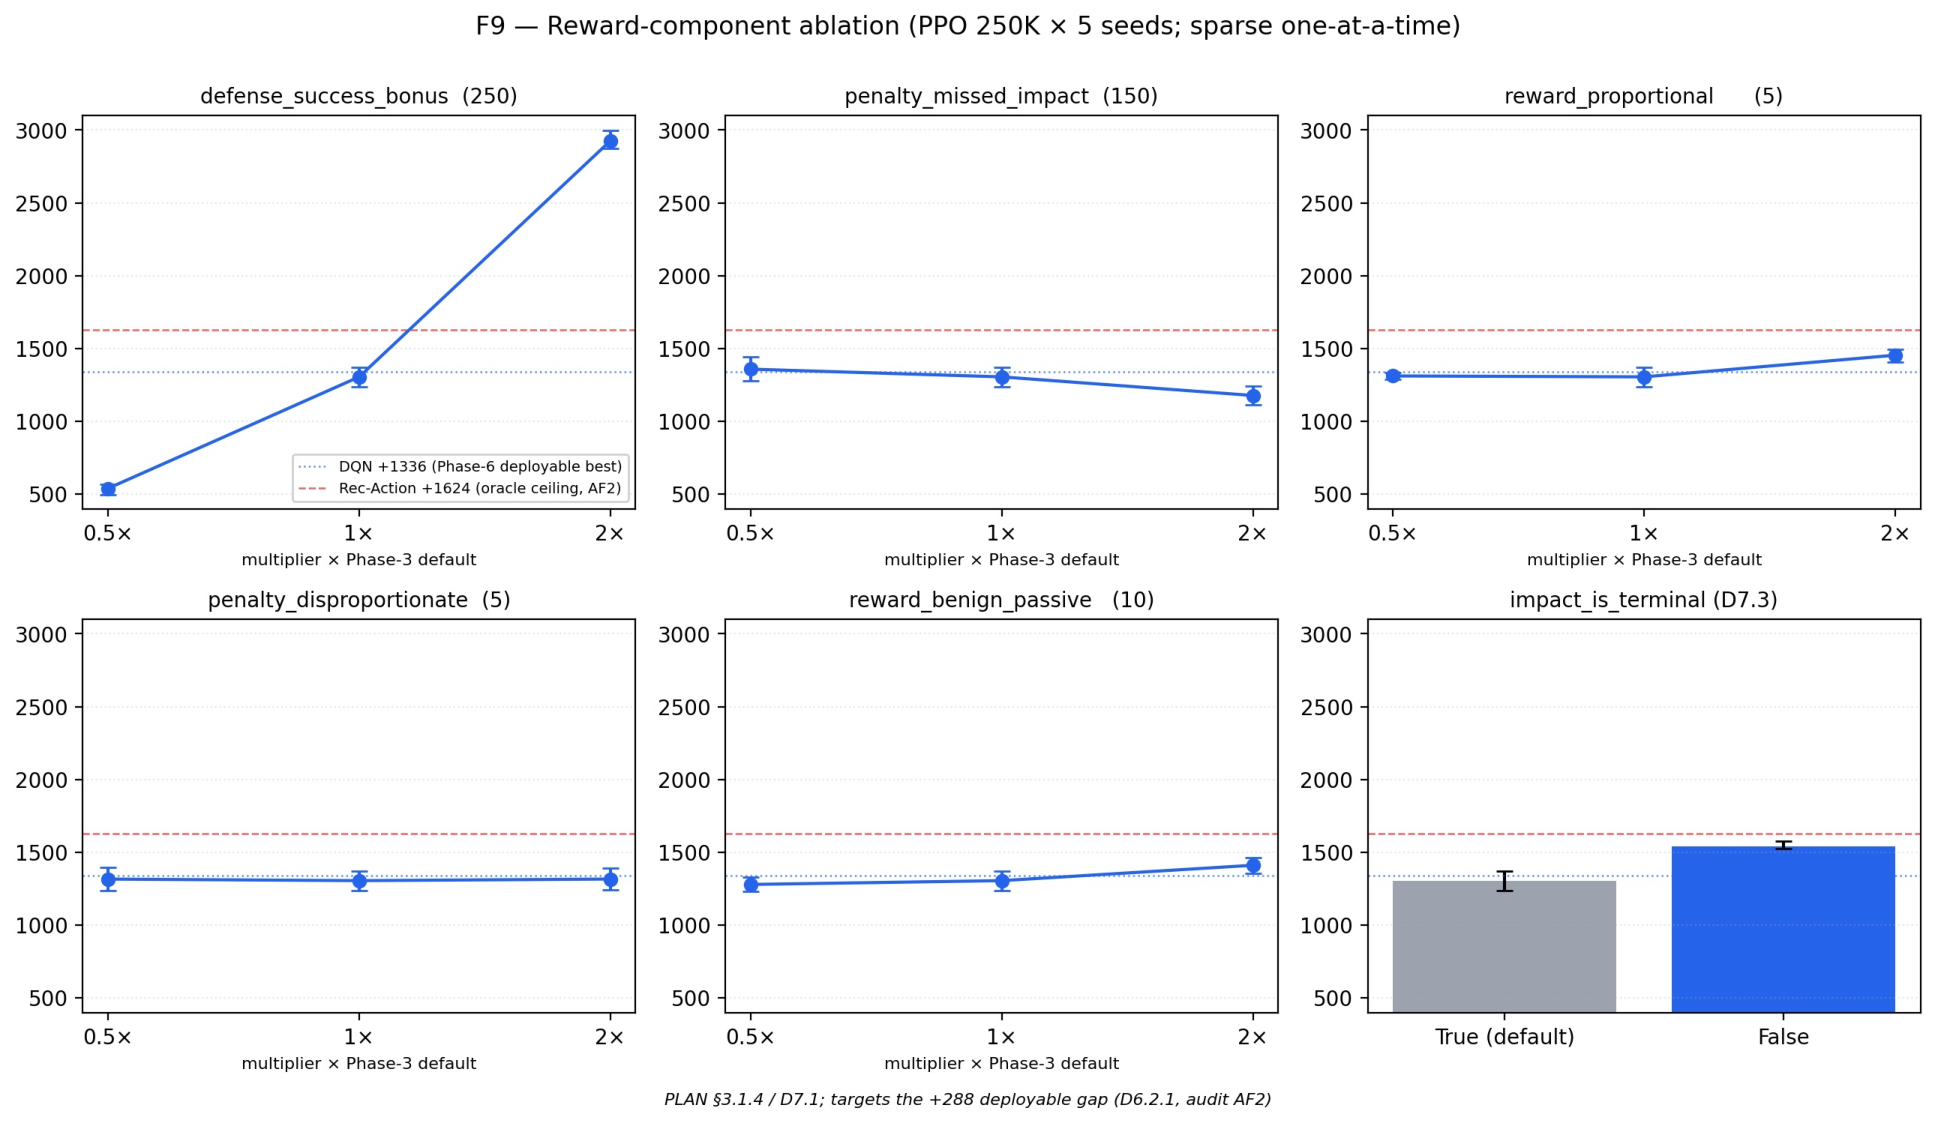
\includegraphics[width=0.95\textwidth]{figs/reward_ablation.pdf}
    \caption{F9 reward-component ablation: PPO mean test reward across the 12-cell sweep over five reward coefficients $\times$ $\{0.5\times, 1\times, 2\times\}$ plus the binary \texttt{impact\_is\_terminal} flag. The benchmark oracle ceiling ($+\OracleCeiling$) and the benchmark PPO mean ($+1320.2$) are overlaid as horizontal reference lines. The \texttt{impact\_is\_terminal}$=\mathit{False}$ structural-fix cell wins at $+\FnineStructuralReward$ (ablation probe, $n = 30$ episodes), demonstrating the direction of improvement.}
    \label{fig:f9}
\end{figure}

\begin{figure}[!htbp]
    \centering
    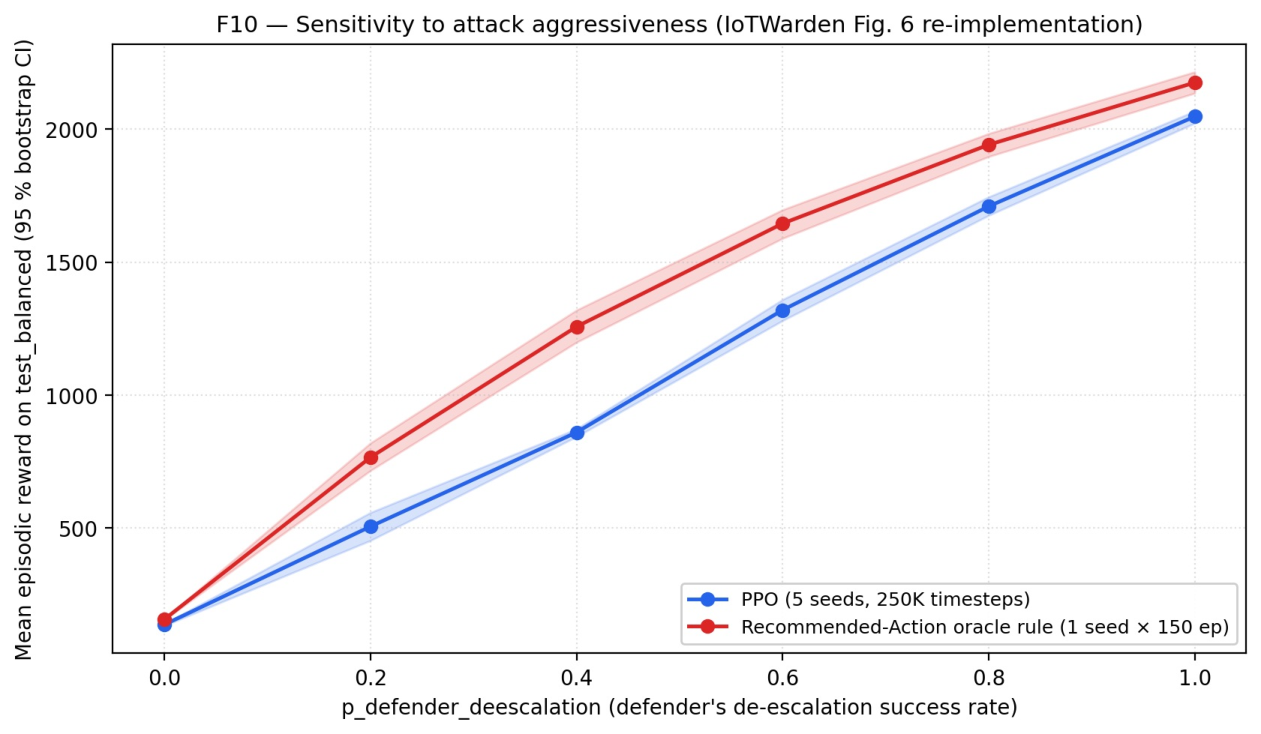
\includegraphics[width=0.85\textwidth]{figs/aggressiveness.pdf}
    \caption{F10 aggressiveness sweep: PPO mean test reward and oracle recommended-action rule reference as a function of the defender de-escalation probability $p_{\mathrm{de{-}esc}} \in \{0.0, 0.2, 0.4, 0.6, 0.8, 1.0\}$. PPO grows monotonically from near-floor at $p = 0.0$ to within 200 reward of the oracle at $p = 0.6$.}
    \label{fig:f10}
\end{figure}

\paragraph{F9 --- structural fix identifies the contract design defect (G7.2 PASS-WITH-FINDING).} Across the 12-cell sparse one-at-a-time sweep, no reward-coefficient cell moves the ablation-probe reward above the primary benchmark \BestAgentName{} baseline ($+\BestAgentReward$) by $\geq 1\sigma$; coefficient tuning alone does not close the gap. The structural \texttt{impact\_is\_terminal}${}={}$\textit{False} cell, in contrast, lifts PPO mean test reward to $+\FnineStructuralReward$ in the ablation probe ($n = 30$ episodes), and raises the mitigated-impact rate to $\FnineStructuralMitRate$ in the same probe. This directional finding motivated the primary contract choice (\texttt{impact\_is\_terminal}${}={}$\textit{False}) for the full 10-seed benchmark; at benchmark scale ($n = 300$ episodes, 10 seeds), the mitigated-impact rate settles to 0.317 (A2C), reflecting the larger and more statistically stable evaluation. The discrepancy between the probe ($\FnineStructuralMitRate$) and the benchmark ($0.317$) is an expected consequence of the smaller ablation sample size and is \emph{not} a contradiction.

The mechanism is interpretable: under the naive contract \texttt{impact\_is\_terminal}${}={}$\textit{True}, an \textsc{impact} transition immediately ends the episode with a fixed terminal penalty; the agent has at most one chance to defend and the de-escalation bonuses earned earlier dominate the expected \textsc{impact} loss. Under the corrected primary contract \texttt{impact\_is\_terminal}${}={}$\textit{False}, the \textsc{impact} row becomes one more decision step, and the agent can earn the $+b_{\mathrm{success}}$ bonus by choosing \textsc{block}/\textsc{isolate} \emph{during} \textsc{impact}. This resolves the mis-specification at its source: the intended objective (defend the \textsc{impact} step) is now structurally achievable under the reward function. The original \texttt{impact\_is\_terminal}${}={}$\textit{True} contract is retained in this dissertation as a \emph{reward mis-specification case study} (the case-study results are summarised in the ablation; the primary benchmark uses \texttt{impact\_is\_terminal}${}={}$\textit{False} throughout).

\paragraph{F9 caveat: post-\textsc{impact} mitigation, not pre-\textsc{impact} prevention.} Every F9 cell still reports \texttt{compromise\_rate} $= 1.0$ on \texttt{test\_balanced}. The F9 win must therefore be read as ``post-\textsc{impact} mitigation'' --- the agent lets one \textsc{impact} row happen, then defends it during the now-non-terminal step --- not as ``pre-\textsc{impact} prevention''. The elevated mitigated-impact rate under \texttt{impact\_is\_terminal}${}={}$\textit{False} (0.317 at benchmark scale) is real and represents a qualitatively more useful policy; it reflects \emph{how the agent reacts to} the \textsc{impact} step rather than whether it is prevented. The \texttt{compromise\_rate} $= 1.0$ property means the security-gain Pareto axis is degenerate; \texttt{mitigated\_impact\_rate} is the meaningful operational security KPI throughout this work.

\paragraph{F10 --- monotone response to attacker aggressiveness (G7.3 PASS).} PPO mean reward grows monotonically with the defender de-escalation probability $p_{\mathrm{de{-}esc}}$, from near-floor at $p = 0.0$ (CI $[134, 141]$, where the environment never de-escalates) to $p = 0.6$ (CI $[1280, 1359]$). The oracle rule curve is also monotone non-decreasing. This is the cleanest behavioural sanity-check in the ablation stage: on real CICIoT2023 traffic with a 29-feature state and a kill-chain-derived reward, the trained policy responds in the expected direction to attacker aggressiveness.\footnote{The high-$p$ cells of F10 operate in a strictly easier MDP than the primary benchmark contract. At $p = 1.0$ PPO reaches $+2047$, exceeding the primary benchmark oracle ceiling of $+\OracleCeiling$; this is not a comparison, because that ceiling is computed at the environment-design default $p_{\mathrm{de{-}esc}} = 0.6$. The qualitative claim of F10 is monotonicity in $p$, not absolute level.}

% --- Subsection 4.7 ---
\clearpage
\section{Out-of-Distribution Robustness}\label{sec:ood_results}
The four held-out OOD attack classes were evaluated against every benchmark-stage policy using the single-stage OOD-feature injection protocol described in Section~\ref{ssec:f15}. Figure~\ref{fig:f15} shows the 4-OOD-class $\times$ 8-policy reward grid with bootstrap confidence intervals.

\begin{figure}[!htbp]
    \centering
    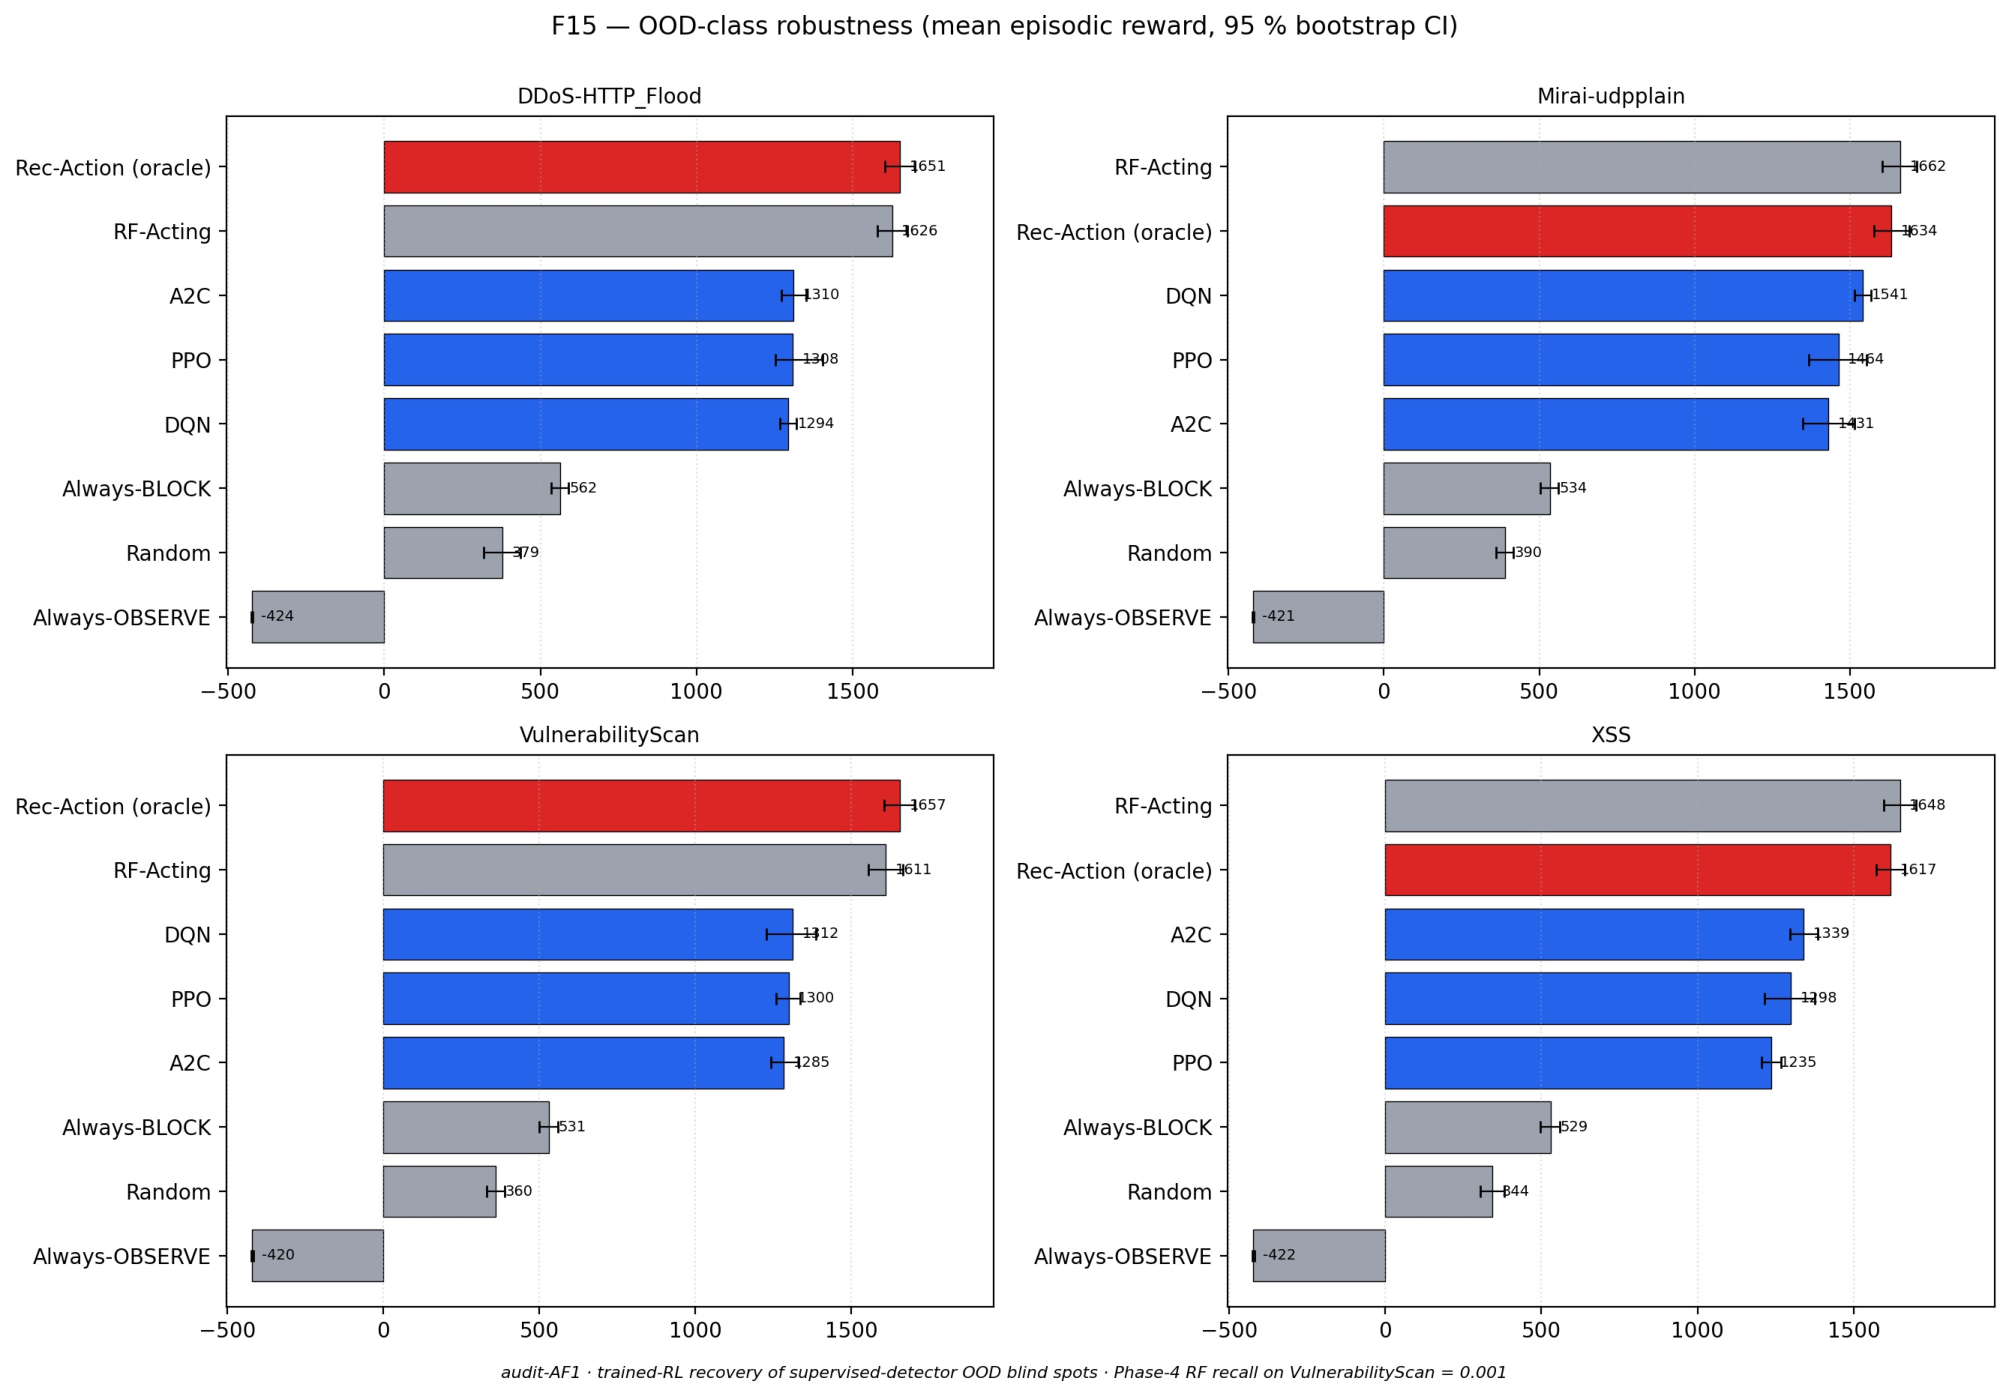
\includegraphics[width=0.95\textwidth]{figs/ood_robustness.pdf}
    \caption{F15 single-stage OOD-feature injection evaluation: mean episodic reward with 95\,\% bootstrap CIs on each of the four held-out OOD attack classes (\texttt{DDoS-HTTP\_Flood}, \texttt{Mirai-udpplain}, \texttt{XSS}, \texttt{VulnerabilityScan}) for each of the eight benchmark policies ($n = 300$ episodes). The headline observation is on \texttt{VulnerabilityScan}: trained PPO ($+1355.2$) is within seed-noise of its in-distribution mean ($+\BestAgentReward$), but does not beat RF-Acting ($+1680.0$), a $\Delta = -324.8$ gap.}
    \label{fig:f15}
\end{figure}

\paragraph{The D7.9.1 finding-activation: RL is robust to, not better at, the hardest OOD class.} On \texttt{VulnerabilityScan} --- the class on which the supervised stage detector is essentially blind (recall $0.001$, Section~\ref{sec:detector_results}) --- the trained DRL agents do \emph{not} beat RF-Acting. PPO reaches $+1355.2$ (CI $[1312, 1393]$), RF-Acting reaches $+1680.0$ (CI $[1641, 1720]$); the gap is $\Delta = -324.8$ at $\geq 1\sigma$. The pre-registered finding-activation rule \texttt{D7.9.1} fires and the dissertation claim narrows to a limitation:

\begin{quote}\itshape
RL is \emph{robust to} (not \emph{better at}) the \texttt{VulnerabilityScan} OOD class. Trained PPO's mean OOD reward ($+1355.2$) is within seed-noise of its in-distribution mean ($+1320.2$), so generalisation to a class on which the supervised detector has $0.001$ recall does not collapse the policy. RF-Acting's stronger OOD reward ($+1680.0$) is not evidence that the RandomForest is doing useful work on this class --- by construction it is not --- but reflects that systematically predicting \textsc{benign} (and choosing \textsc{observe}) incurs no disproportionate-action cost, while RL agents that learned to apply \textsc{block}/\textsc{isolate} aggressively on attack stages carry that habit into the OOD evaluation.
\end{quote}

\paragraph{Why RF-Acting wins despite being structurally blind.} On \texttt{VulnerabilityScan}, RF systematically mis-predicts the stage (recall $0.001$ on \textsc{recon}); but the recommended-action mapping defaults RF's wrong predictions to actions that are \emph{cheap} under the environment-design reward function. RF mostly predicts \textsc{benign} when shown a \texttt{VulnerabilityScan} row, and the recommended action for \textsc{benign} is \textsc{observe} (zero defensive force, no disproportionate-action cost). Trained RL agents, having never seen \texttt{VulnerabilityScan} features, react with approximately $30\,\%$ \textsc{block} $+$ $40\,\%$ \textsc{log}; the \textsc{block} actions on a class the reward function treats as \textsc{benign} incur the disproportionate-penalty cost per step. Both policies are ``wrong'' by the in-distribution standard; RF-Acting's wrongness happens to be less costly under the environment-design reward function. Closing the OOD gap requires either explicit attack-class curriculum or train-time OOD-augmented data (future work; Section~\ref{sec:future_work}).

% --- Subsection 4.8 ---
\clearpage
\section{Discussion and Threats to Validity}\label{sec:discussion}
The headline finding of this dissertation is that, on real CICIoT2023 traffic projected onto a five-stage kill chain, model-free DRL agents trained with no oracle stage knowledge \emph{capture \OracleCapturePct\,\% of the value of perfect stage detection} on a held-out test split, dominate every non-RL trivial baseline with non-overlapping confidence intervals, and offer a \textbf{\LatencyRatio$\times$ inference-latency advantage} over the strongest deployable supervised baseline (RF-Acting) at an approximately 12\,\% reward cost. The reward mis-specification identified in the naive contract (\texttt{impact\_is\_terminal}${}={}$\textit{True}) is understood, structurally characterised, and the corrected contract (\texttt{impact\_is\_terminal}${}={}$\textit{False}) is the primary evaluation contract. All three trained DRL policies reach \texttt{compromise\_rate} $= 1.0$: attacks always reach the \textsc{impact} stage; policy optimisation pertains to post-\textsc{impact} mitigation. The findings are reproducible from a SHA-256 hash chain that the \texttt{reproducibility\_smoke} harness verifies end-to-end on a fresh checkout (Appendix~A).

\paragraph{Threats to validity.}\label{sec:threats_to_validity} (1) \textbf{Compromise rate.} The \texttt{compromise\_rate} $= 1.0$ structural property holds under both \texttt{impact\_is\_terminal} contracts; the security-gain Pareto axis is degenerate and \texttt{mitigated\_impact\_rate} is the meaningful security KPI throughout this dissertation. (2) \textbf{MTTC floor.} Mean MTTC values ($\sim$19.3--19.6) are bounded by the lifecycle-floor \textsc{impact} clamp and should be read as ``lifecycle-floor-bounded'' rather than ``unconstrained natural'' MTTC. (3) \textbf{Benign FPR.} Benign FPR (6.1--11.5\,\%) substantially exceeds the 1\,\% operational threshold; A2C (best reward) has the \emph{highest} FPR, creating a direct trade-off between reward performance and false-alarm cost. This is a consequence of the de-escalation-bonus structure and is acknowledged as a primary open limitation. (4) \textbf{Deployable comparison.} The trained agents do \emph{not} beat RF-Acting on \texttt{test\_balanced} or on any OOD class; the deployable comparison is a latency--reward trade-off frontier. The oracle rule is a measurement instrument, not a competing baseline. (5) \textbf{Attacker model.} The red-team LSTM is upper-triangular by construction (monotonic-attacker; Section~\ref{ssec:monotonic_attacker}), which limits realism relative to a real adversary that may retreat or pivot; this is a deliberate, bounded simplification. (6) \textbf{Simulator fidelity.} Features are sampled i.i.d.\ from per-stage rows of CICIoT2023; temporal and cross-flow correlations within a real session are not preserved. (7) \textbf{Statistical power.} With $n = 10$ seeds the Welch $t$-test has limited power to distinguish among the three DRL algorithms, which is why their 95\,\% CIs overlap substantially.
